% This file is isea.tex.  It contains the formatting instructions for and acts as a template for submissions to ISEA 2015.  It is based on the ICCC  formats and instructions.  It uses the files isea.sty, isea.bst and isea.bib, the first two of which also borrow from AAAI IJCAI formats and instructions.
% Modified from ICCC.tex by B. Bogart

\documentclass[letterpaper]{article}
\usepackage{isea}
\usepackage[pdftex]{graphicx}
\usepackage{times}
\usepackage{helvet}
\usepackage{courier}
\usepackage{listings}
\usepackage{appendix}
\usepackage{xcolor} % Optional, for color customization
\definecolor{codegreen}{rgb}{0,0.6,0}
\definecolor{codegray}{rgb}{0.5,0.5,0.5}
\definecolor{codepurple}{rgb}{0.58,0,0.82}
\definecolor{backcolour}{rgb}{0.95,0.95,0.92}

\lstdefinestyle{mystyle}{
    backgroundcolor=\color{backcolour},
    commentstyle=\color{codegreen},
    keywordstyle=\color{magenta},
    numberstyle=\tiny\color{codegray},
    stringstyle=\color{codepurple},
    basicstyle=\ttfamily\scriptsize,
    breakatwhitespace=false,
    breaklines=true,
    captionpos=b,
    keepspaces=true,
    numbers=left,
    numbersep=5pt,
    showspaces=false,
    showstringspaces=false,
    showtabs=false,
    tabsize=2
}
\lstset{style=mystyle}

\usepackage[numbers]{natbib}
\pdfinfo{
/Title (Shared Memory Pool for Representors)
/Author (Netdev Conference 0x18, 2024)}
% The file isea.sty is the style file for ISEA 2015 proceedings.
% reference: epoll paper: Busy Polling: Past, Present, Future
% https://netdevconf.info/2.1/papers/BusyPollingNextGen.pdf
% reference: ./Documentation/networking/representors.rst
% old slides about eswitch
% https://www.netdevconf.info/1.2/slides/oct6/04_gerlitz_efraim_introduction_to_switchdev_sriov_offloads.pdf


\title{Shared Memory Pool for Representors}
\author{William Tu, Michal Swiatkowski, and Yossi Kuperman\\
Nvidia and Intel\\
witu@nvidia.com, michal.swiatkowski@intel.com, yossiku@nvidia.com\\
\newline
\newline
}
\setcounter{secnumdepth}{0}

% due deligent https://lore.kernel.org/netdev/39dbf7f6-76e0-4319-97d8-24b54e788435@nvidia.com/
%
\begin{document} 
\maketitle
\begin{abstract}
Representor netdevs are special objects that controls the switchdev
virtual port, which is the reprensentee. It configures administratively
of the virtual port, as well as provides the slow path for traffic which
does not hit any offloaded fast-path rules in the switchdev.
%Packets transmitted by the representor netdev are delivered to the vport;
%and packets tansmitted by the vport are received by the representor
%netdev, if it fails to match any offload rule.
When scaling to thousands of vports, a correpsonding thousands of
representor netdevs are created, usually one vport has one representor
netdev. With modern NIC containing advanced offload capabilities % what's intel's flow table size and offload cap?
and increasing flow tale size, the role of representor netdev becomes
lightweight but also critial. It processes the first couple of packets
from a new connection, extracts the protocol information, and insert
into the NIC hardware for subsequent packets to hit fast-path rules. 

Creating thousands of representor netdevs becomes resource heavy for
just handling the connection setup, especially for the SmartNIC or
DPU (Data Processing Unit). A Nvidia Bluefield-2 only contains 16GB
of memory, but with one thousand representor netdev can use up to
12GB of RX memory buffer. A trivial solution is to trade-off the
performance by reducing the RX queue entries, usually 1024, to a
smaller number such as 64. The paper proposes saving these representor
netdev's memory buffer by using a share memory pool, and a generic
configuration UAPI through devlink for user to adjust the pool size. 
 
\end{abstract}
%fig1: 
%fig2:

\section{Introduction}
Modern network devices support advanced switching and offloading
capabilities, called switchdev mode. In switchdev mode, users can
create multiple virutal ports, or vports, through sysfs and assign
vports to virtual machine or containers. The switchdev mode includes
PF (Primary Functions of a PCIe device, with full access to the device's
capabilities. PFs can manage multiple types of vports, including
VFs (Virtual Functions) and SFs (Sub/Scalable Functions) and PF is
responsible for the control and configuration of the device.
The switchdev design follows the split model: a fast-path and slow-path, shown in Figure~\ref{fig:arch}.
A NIC with advanced offload capability and flow table rules is
the fast-path, while a corresponding software switch that handles
initial flow rule setup, or the miss traffic processing, is considered the
slow-path. Different vendors such as Nvidia Connect-X or Intel ICE
supports different offload capabilities, but they follow similar
software slow-path design, with OVS or Linux bridge attached with
the slow-path vport, running either on host CPUs or SmartNIC/DPU
ARM cores.

The slow-path ports that handles miss traffic is called representor
netdevs, registerd as a regular Linux ethernet device and is responsible
for administratively configurations of the fast-path vport, ex: SF or VF.
In typical use cases, representor netdev and its representee, vport,
are 1-to-1 mapping: a VF/SF has a its own netdev for fast-path traffic,
and another representor netdev for slow-path traffic.
Such a design is reasonable with tens or hundred-ish vports but when scaling
to thousands of VFs or SFs, the memory resource becomes a limiting factor.
For example, assuming each RX queue has 1024 entries, and each entry
pointing to a 4K-sized page. Assume the netdev has 4 RX queues (controlled
by ethtool -L combined), a netdev will consume 4 * 4K * 1024 = 16MB.
With 1k representor netdevs, the memory consumption can grow
to 16GB (16MB * 1024). We found that majority of memory comes from
the RX memory buffers~\cite{jakub}, i.e., the pre-allocation of RX queues
that handles burst of incoming traffic.

% explain what's rx buffer
The pre-allocation of RX queues and buffers are configured by Linux
ethtool -G option, with different vendors setting different default
value. Nvidia MLX5, by default, pre-allocates 1024 entries in each of
its RX queues, with each entry pointing to a MTU-sized buffer or a page
(without striding RQ). For Intel ICE, it's also 1024 entries. % need to check
A trivial solution is to reduce the number of RX queue entries of
representor netdevs, for example, from 1024 to 64 (the minimum of NAPI
budget). Although this saves memory but a burst of traffic over 64 packets
will be dropped, causing longer connection offload setup time.

The paper describes the recent solution done by a couple vendor drivers.
Instead of having one representor netdev per SF or VF, redirect all
the slow-path traffic from all VFs/SFs to a single netdev, usually PF or
uplink representor. As a result, the PF's RX queue receives all slow-path
traffic from all other representors. In other word, all representors
share the same RX queue memory pool provided by PF. The idea of using PF's
RX qeueu as a shared memory pool is currently used by Intel ICE, Netronome,
Broadcom bnxt, and SFC~\cite{survey}.
%And this saves lots of memory because slow-path traffic is redirected to
%PF, representors no longer needs to create its own RX queues and buffers.
Experimental result shows that we can create 1K SFs and having the 1K
representor netdev sharing its RX queue and buffers with PF. Although
it saves lots of memory, but without large and real traffic experiment,
it's hard to measure the performance impact of PF-based sharing memory
pool versus no shared design. In addition, we found that when using share
memory pool, a VM using a VF/SF can easily monopolize the entire memory
pool, making another VM with VF/SF zero bandwidth. For example, a VM
running dpdk-testpmd to send 4Mpps of UDP traffic can easily use the
entire PF's shared memory pool, causing all the rest of VM starvation.

The situation is similar to buffer management problem in shared-memory
packet switches, where the hardware switch has a shared memory pool
for all its ports and how to guarantee both the performance and
fairness~\cite{devlinksb, queuelength}. The solution couldn't apply to
our case because it's slow-path traffic, all the hardware traffic
control or QoS features are not available.

We describe more background in later section, design of the PF memory
sharing pool, solution to the fairness problem, and finally some performance
number. The paper has the following contributions:
\begin{itemize}
    \item Present the memory consumption requirements for scaling to
          thousands of devices.
    \item Describe the existing solutions from different driver vendors,
          using shared RX queue provided by PF.
    \item Propose a solution to save memory per RX queue by dynamically
          post and reclaim pages.
    \item Propose a solution using a shared page pool for all netdevs,
          with inherent fairness mechanism.
\end{itemize}

\begin{figure}[h]
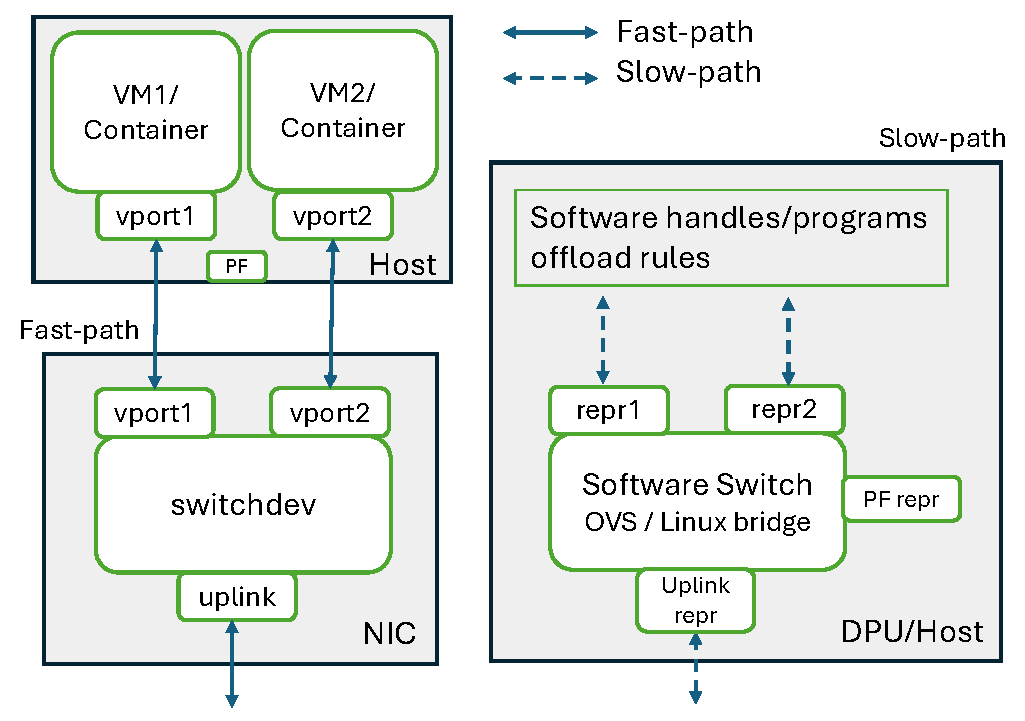
\includegraphics[width=3.4in]{arch.pdf}
\caption{The fast and slow path model. The switchdev in NIC is the fast path handling
hardware offloaded traffic among VFs/SFs, and the DPU which contains representor netdevs and software switch handles the slow path traffic.}
\label{fig:arch}
\end{figure}

%This post an important question: how much memory buffer does a representor
%netdev needs to pre-allocate for bursty traffic?
\iffalse
most of these representor netdevs' RX DMA memory
is idle when flows are forwarded directly in hardware to VFs.
In the recent case of smartnic or DPU (data processing unit) such as
Nvidia BlueField and Intel IPU, only the VFs and SFs and a light-weight PF
is exposed to the host side, the PF and representors are created in the
embedded CPU of the smartNIC.
The SmartNIC usually has less memory resources, Nvidia BlueField 3 has
32GB and Intel IPU has NGB, which makes the memory resource more precious.

In this talk we address the memory utilization challenges in DPU, by
first going through all existing solutions in different vendor drivers,
intel, nvidia, broadcom, netronme, and sfc. And we present the shared
memory pool design and implementation.
We should that by sharing the memory 
\fi

\section{Background}

\subsection{Eswitch and Switchdev Mode}
An eSwitch, or embedded switch, is a hardware component within modern network
controllers, such as the Intel® Ethernet Controller E810. It is also known as
a Virtual Ethernet Bridge (VEB). The eSwitch is managed by the Physical Function (PF)
driver of the Ethernet or in the case of SmartNIC, managed by the ECPF (Embedded CPU
s PF) that runs in the smartNIC's core. Eswitch can operate in two modes:
Legacy mode and Switchdev mode.

Legacy mode operates based on traditional MAC/VLAN steering rules. Switching
decisions are made based on MAC addresses, VLANs, etc. There is limited ability
to offload switching rules to hardware.
On the other hand, switchdev mode allows for more advanced offloading
capabilities of the E-Switch to hardware. In switchdev mode, more switching
rules and logic can be offloaded to the hardware switch ASIC, for example
push and pop tunneling protocol, connection tracking, etc.
This mode requires a slow path, software components such as OVS or
Linux bridge, and representor netdevices that handle miss traffic,
the flows that can not be offloaded or miss the hardware flow table
lookup, the slow path of VFs or SFs of the device.
% $$:`Documentation/networking/switchdev.rst <switchdev>` and
%:ref:`Documentation/networking/representors.rst <representors>`.
% devlink dev eswitch show
% devlink dev eswitch set mode switchdev
% need to disable OVS hwoffload
% so it's the iperf TX traffic on VF port that's going to overflow the PF's rxq

\subsection{Representors}

A vport can be PFs (used by administrator), or VFs or SFs (assigned to VMs
or containers). When the hardware offload table is empty, all packets are 
processed by the slow path. Representor netdev and vport are like a linux
pipe, shown in Figure~\ref{fig:pipe}: packets transmitted by the representor
netdev are delivered to its vport; packets transmitted by the vport are
received by the representor netdev, if it fails to match any offload rule.

% an end-to-end example
For example in Figure~\ref{fig:arch}, VM1 would like to setup a new TCP
connection to VM2. The first TCP syn packets sent from VM1 will miss the
NIC switchdev's flow table, due to no match, and arrives at the receive
queue of vport1's corresponding representor netdev, repr1.
OVS in this case, with hardware-offload enabled, will parse the protocol
and insert an offload rule, using Linux tc-flower interface.
In addition, OVS also forwards/sends the packet to the repr2 port, which
will deliver the packet to vport2's receive queue at VM2.
While VM2 receives the TCP syn from VM1, VM2 replies with SYN+ACK, and
again goes through the slow path. Until the connection is established
and flow rules are in NIC's flow table, the TCP data stream will be
going through the fast-path in NIC, and OVS in DPU no longer involves
in any packet processing.

Note that the behavior of the slow-path (representor ports and software
switch) should be the same as fast-path (vports and switchdev).
And because representor and vport are acting like pipe, so an OpenFlow
rule on a representor netdev applies to a packet on its
receive path is the same as it applies on vport's transmit path.
\begin{figure}[h]
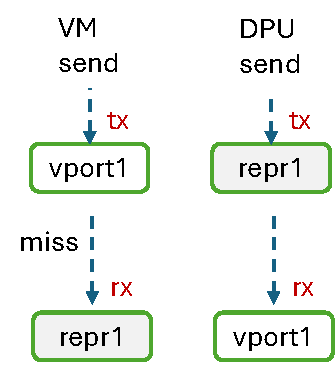
\includegraphics[width=1.5in]{pipe.pdf}
\centering
\caption{The vport and representor: packets transmitted by the representor 
netdev are delivered to its vport; packets transmitted by the vport are
received by the representor netdev, if it fails to match any offload rule.}
\label{fig:arch}
\end{figure}

\iffalse
When the system boots, and before any offload is configured, all packets from
the virtual functions appear in the networking stack of the PF via the
representors.
The PF can configure standard Linux forwarding between representors, the uplink
or any other netdev (routing, bridging, TC classifiers).
Thus, a representor is both a control plane object (representing the function in
administrative commands) and a data plane object (one end of a virtual pipe).
\fi

\subsection{Memory Pre-allocation}
Network device drivers need to buffer the incoming packet from network,
by pre-allocating memory for received packets. Once the packets arrive,
NIC can DMA a batch of packets into these pre-allocated buffers,
potentially hundreds of them, before the host CPU is notified/kicked in
by interrupts to process these packets.
For performance reason, NIC contains multiple channels with each channel
represents an NAPI context and an IRQ to kick in to process rx packet.
Usually the number of channel is the same as number of CPU that involves
in packet processing.
In typical case, a channel contains a packet receive queue,
and by default the RX queue contains several entries, with each entries
point to a packet buffer. So the amount of pre-allocated memory for RX
is a product of buffer size * number of queues * queue depth.
A typical example of a data center server with 64 cores would be:
4k * 64 queues * 1k entries = 256MB.

Note that the queue depth, or the number of entries in RX queue, is
not only for tolerating the burstness of traffic, but also the CPU
processing time/jitter of a packet. When CPU is under heavy loading,
a packet arriving RX interrupt might not be able to immediately
kick in the CPU to process packets. Thus a deeper queue depth can
avoid packets being dropped.
In addition, each packet usually has different processing time.
The time for CPU to process a TLS packet is definitely longer than
an ARP packet. Thus, a deeper RX queue also helps avoiding packets
dropped due to intermittently longer packet processing time.



However, memory in not cheap, especially when scaling to 1K devices
and with 1k representor netdevs in DPU. And having several GBs of
pre-allocated memory idle just waiting for a burst of traffic
or even unused when the low traffic volume is a huge resource waste.
We discuss our solution in later section.

\section{Design}
% table here shows existing driver's implementation~\cite{buffersize}
We'd like to support 1K of SFs/VFs with representor netdevs
on DPU, with the following requirements: 1) 1k netdev creation time
around 10 minutes, including configurations and bringing the device up,
2) memory consumption of DPU system is within
system limit, and 3) all the VFs/SFs representor get fair share
of receive memory buffer, which leads to fair share of bandwidth.
With that in mind, we describe three solutions: Shared RX queue with PF,
Adjustable RX queue, and Adjustable RX queue with meters. 

\subsection{Shared RX Queue with Service Netdev}
\begin{figure}[h]
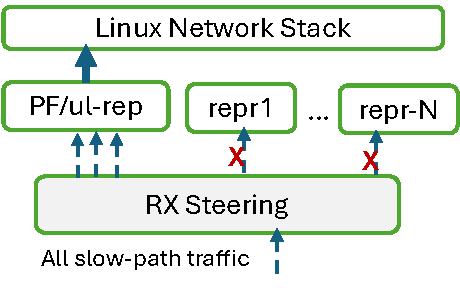
\includegraphics[width=2in]{design1.pdf}
\centering
\caption{Shared RX Queue: A PF/uplink-representor netdev receieves all slow-path traffic
for other representors, and reconstructs their skb and passes to upper
network stacks.}
\label{fig:arch}
\end{figure}

Since the representor netdev only handles the miss traffic or first
few packets for connection setup, existing solution is to assign a
a dedicated service netdev for handling \emph{all} traffic from other
representors. This dedicated service netdev acts like an intermedia
multiplex layer, it sees all slow path traffic from all the
reprensentors, and lookup an internal data structure to identify the
orignal source of VF/SF, reconstruct the skb->dev to the correct
orignal netdev, and pass up kernel stack. As a result, the representor
netdev no longer sees packets and no need to allocate RX queue.

Service netdev can be any netdev, but commonly used are PF or the uplink
representor netdev. For Intel ICE driver, PF is used to receive all other
reprensetor's traffic.
Different vendors have different design, but in general, the device
driver needs to do the following:

%Recall that in Figure~\ref{fig:pipe} the representor and vport are like pipe.
\begin{itemize}
\item RX hardware steering: instead of sending slow-path traffic to
each individual representors, the NIC needs to steer/redirect all
slow-path traffic to the service netdev, and mark the packet's orignal
vport information, vport\_id, in metadata or packet buffer.
\item RX software: the service netdev now sees all traffic including
others arriving at its RX queues. It needs to keeps a map of vport\_id
to the packet's original netdev struct. By extracting the vport\_id
from metadata, the orignal netdev is restored to sk\_buff and continue
kernel network stack. The representor netdev no longer allocates memory
for RX queues and buffers.
%it is able to distinguish which vport the packet
\item TX: because the vport and representor act like a pipe, the service
netdev need to know which vport's RX queue the packet should be \emph{send}
to. Drivers can use the dst\_entry of skb, or other per-packet metadata
field, and rely on internal switch to deliver the packet to the vport.
\end{itemize}

\emph{pros and cons:}
The shared rx queue solution saves lots of memory by redirecting
all traffic to service netdev, because it consumes only one service
netdev's memory. Depending on number of SF/VFs and traffic volume,
users need to configure two parameters of service netdev:
\begin{itemize}
    \item the number of RX queues should increase to decrease the chance
    of multiple flows from multiple vports rxhash to the same queue.
    (ethtool -L combined) Today, the max RX queue is usually limited by
    number of CPUs.
    \item the RX queue depth should increase to absorb more traffic
    burst from multiple vports. (ethtool -G rx)
    \item reduce the NAPI schedule delay, which means napi can process
    packets as soon as possible when packets arrived, can reduce the queue
    depth grows to fast. (I don't know any tool to do this)
\end{itemize}

The design is simple to implement, but we found that it suffers from
a fairness issue. A single high volume sender, ex: dpdk-pktgen,
sending to its vport and arrives at slow path, can easily consume all
the buffers in the service netdev's RX queue, making other representor's
traffic being dropped. An example setup script to show case the issue
using OVS and Linux bridge is provided in Appendix.

\subsection{Adjustable RX Queues}
Since sharing the RX Queues of PF or uplink representor suffers fairness
issue, another solution is to {\em not} sharing the RX queue. That is, each
representor acts like a regular netdevs, with its own RX queues and RX buffers.

To save memory, for every queue in every netdev, instead of doing the
static RX queue allocation, which always allocating to \emph{full} RX queue
depth, we propose to dynamically adjust RX queue.
For example, an mlx5 driver, by default, always tries to allocate to
full 1024 rxq buffers. Instead, the following logic is applied when
a driver is receiving packets in its NAPI context:
\begin{itemize}
    \item NAPI busy: allocate buffers and refill to full queue depth.
    \item NAPI interrupt: allocate buffers and refill to low watermark if
    current queue depth is lower than low watermark
    \item NAPI interrupt: do not allocate and refill if current queue
    depth is higher than low\_watermark.
\end{itemize}

We set the low\_watermark to be 128 (2 * NAPI\_BUDGET). 
The low\_watermark means the minimal available buffers to handle the
worst case of traffic burst. At driver initialization time, all queues
are allocated only up-to the low\_watermark. Once the first burst
of traffic arrives, users might see more packets dropped compared
to full rxq depth allocation (1024). Fortunately, a NAPI busy state will
trigger driver to refill to its full rxq depth, making the performance
impact minimal. In this design, we pay the performance price to save
memory. The first burst traffic of a connection see more packets dropped,
and once in NAPI-busy, the driver acts the same as static RX queue
allocation.

The high\_watermark is the max RX queue depth, which is the same value
set in static allocation, the rxq depth set by (ethtool -G rx)

Such a design saves memory at driver initialization, as well as the
NAPI-interrupt
state will slowly return page back to kernel due to packet arrives but
driver does not allocate and refill. However, what if an rxq is in
NAPI-interrupt, but there is no packet arrived to trigger returning
pages to system? Then driver needs to detect and drain the RX queue
back to the low\_watermark.

\textit{pros and cons:} 

\subsection{Adjustable RX Queues with Shared Page Pool}

Currently each queue creates its own kernel page pool, and in NAPI, refilling
the RXQ buffer by getting a page pool entry from its own per-queue page pool.
When scaling to thousands of representor netdevs, there is no guarantee that
all the representor netdev gets fair share of system memory. That is, the late
coming netdevs might see system out-of-memory for initializing its RXQ ,
even with the Adjustable RX Qeueue design.

We propose shared page pool, a layer of page pool that runs on top of current
Linux page pool APIs. The shared page pool supports for a group of netdevs
to register as user, and the shared memory pool fairly allocate memory for
each users based on the its current usage and total available memory in
the pool.

Figure~\ref{fig:design3} shows the idea.
Assume N representor netdevs, each has one rxq. In the beginning, the master
netdev, PF or uplink representor, creates the shared page pool, and join
itself into the pool. The netdevs created later join the shared page pool,
by registering itself to the pool, can call the alloc and free API to
returns the page into shared pool. We assume \emph{no lock} is required,
by creating the shared page pool per-CPU NAPI context, which NAPI scheduler
will guarantee not scheduling two NAPIs poll sharing the same pool on different
core.

We define the following C APIs:
\begin{verbatim}
# Uplink representor creates the page pool,
# return the handler of shared pool
spp = shared_pp_create(
    max_num_devs, page_pool_size, …);

# Return a user id for registerd user
spp_uid1 = shared_pp_join(spp, netdev-rep1,
    qid, threshold);
spp_uid2 = shared_pp_join(spp, netdev-rep2,
    qid, threshold);

# Representor NAPI processes packets and
# refills, and bounded by max_usage, return
# -ENOMEM if overflow
shared_pp_dev_alloc_page(spp, spp_uid1);
shared_pp_dev_alloc_page(spp, spp_uid2);
shared_pp_put_page(spp, spp_uid1);

#Leave the share page pool
shared_pp_leave(spp, spp_uid1); 
\end{verbatim}

The shared memory pool enforces a max number of allocated buffer for each user.
We take the idea from Shared-MemoryHardware Switch~\cite{sharedswitch}
For each netdev rxq requesting N memory, there is a limitation of
current max rxq depth = alpha * free buffer.
      
When page pool is under memory stress, the 
The max usage:

The shared page pool allows multiple netdev queues to
allocate memory for its own queues and throttle/reject the netdev n


\subsection{Adjustable RX Queues with Hardware meters}

%\subsection{Nvidia mlx5 driver}
%\subsection{Intel ice driver}
%\subsection{Devlink Interface}
%\subsection{dynamic buffer allocation}
\section{Challenges}
\section{Thanks}

\subsection{Length of Papers}
A variety of paper lengths will be accepted under different categories. Please note that submission lengths must be all inclusive (including references, biographies and acknowledgements).
\begin{itemize}
\item Long paper submissions can be up to 8 pages in the ISEA2015 template format.
\item Art and Research short paper submissions can be up to 4 pages in the ISEA2015 template format.
\item Extended abstract submissions can be up to 2 pages in the ISEA2015 template format.
\item Round tables and square panel submissions can be up to 2 pages in the ISEA2015 template format.
\item Institutional presentation submissions can be up to 2 pages in the ISEA2015 template format.
\end{itemize}

\section{Style and Format}
Templates that implement these instructions can be retrieved electronically at {\small \tt http://isea2015.org}

\begin{figure}[h]
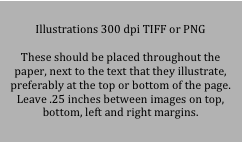
\includegraphics[width=3.31in]{figure.png}
\caption{This is an example of figure caption. Note that all figures, and tables are to be referenced in the text. \copyright Respect Copyright.}
\end{figure}

\subsection{Abstract}

The title ``Abstract'' should be 10 point, bold type, centered at the beginning of the left column. The body of the abstract summarizing the thesis and conclusion of the paper in no more than 200 words should be 9 point, justified, regular type.

\subsection{Text}

The main body of the text immediately follows the abstract. Use 10-point type in {\em Times New Roman} font.

Indent when starting a new paragraph, except after major headings. 

\subsection{Headings and Sections}

When necessary, headings should be used to separate major sections of your paper. (These instructions use many headings to demonstrate their appearance; your paper should have fewer headings.

\subsubsection{Section Headings}

Print section headings centered, in 12-point bold type in the style shown in these instructions. Your body text should be 10 point, justified, single space. Do not number sections.

\subsubsection{Subsection Headings}

Print subsection headings left justified, in 11-point bold type and mixed case (nouns, pronouns, and verbs are capitalized). They should be flush left. Your text should be 10 point, justified, single space. Do not number subsections.

\subsubsection{Subsubsection Headings}

Print subsubsection headings inline in 10-point bold type. Do not number subsubsections.

\subsubsection{Special Sections}

You may include an unnumbered acknowledgments section, including acknowledgments of help from colleagues, financial support, and permission to publish.

The references section is headed ``References,'' printed in the same style as a section heading. A sample list of references is given at the end of these instructions.  Note the various examples for books, proceedings, multiple authors, etc. 

\subsection{Footnotes}

If footnotes are necessary, place them at the bottom of the page in 9-point font. Refer to them with superscript numbers.\footnote{This is how your footnotes should appear.} Separate them from the text by a short horizontal line. 

\subsection{Itemized Lists}

Itemized lists shall use the en-dash as item. Let’s take the case of URL, automatic links and punctuation as an example:
Turn off the automatic linking feature for URLs in Word.

Quotations: For direct quotations remember to use ``double inverted commas.'' Quotations must be carefully transcribed and accurate. 

Periods and commas go inside quotation marks. This applies to ``double inverted commas,'' as well as single `inverted commas,' and to the use of a full stop as in the ``following example.'' 

Parenthesis: When an entire sentence is enclosed in parentheses, the punctuation mark belongs inside the closing parenthesis as in this example: applying this may be difficult at times. (We think it is important.)

\begin{itemize}
\item The punctuation mark belongs outside the closing parenthesis if the brackets are within the sentence as in this example: applying this may be difficult at times, but good results are guaranteed (and this is important).
\item Use en dashes with spaces -- like this -- to set off phrases. En dashes are moreover placed between digits to indicate a range (1--10 October; pp. 25--30). You can type an en dash with ALT + 0150 (in the numeric keypad) in Windows, or OPTION + HYPHEN in Mac.
\end{itemize}

\subsection{Quotations and Extracts}
Indent long quotations and extracts by 10 points at left margins.

\section{Acknowledgments}
The preparation of these instructions and the \LaTeX{} and Word files was facilitated by borrowing from similar documents used for ICCC proceedings.

\begin{figure*}

\includegraphics[width=\textwidth]{two-column-figure.png}
\caption{Example of a double-column figure with caption. \copyright Respect Copyright.}
\end{figure*}

\section{Bibliography}
The title ``Bibliography'' should be 12 point, bold style, centered. Using 9 point, regular type, list your bibliography in alphabetical order by family name, after the references. The difference between a reference list and a bibliography is that in your references, you list all the sources you directly referred to in the body of your writing in numerical order, whereas a bibliography includes an alphabetical listing of all those authors and sources that you have consulted while writing your essay. Use the same format as for the references otherwise. Those using Latex will follow the usual cite command format \cite{boden92}.

\section{Author(s) Biography(ies)}
The title ``Author(s) Biography(ies)'' should be 12 point, bold style, centered. Using 9 point, regular type, biographies should be no longer than 150-word count.

\section{Questions?}
% discussion
% NAPI budget, net_dim, API
% why hardware and software TC QOS doesn't work

For technical questions about Microsoft Word formatting please seek online tutorials. For other questions about your manuscript please contact: {\tt ISEA2015-info@sfu.ca}

\bibliographystyle{isea}
\bibliography{isea}
\section{OVS Script} \label{sec:bash_script}
\begin{lstlisting}[language=sh, caption={Bash Script for Database Backup}, label={lst:bash_script}]
#!/bin/bash

# similar setup for Linux bridge, but disable HW offload by setting aging=0
PF1=eth2
VFREP1=eth4
VFREP2=eth5
VF1=eth6
VF2=eth7
NS1=ns1
NS2=ns2
NS3=ns3
NS4=ns4
SF1=enp8s0f0s88
SF2=enp8s0f0s99
SFREP1=en8f0pf0sf88
SFREP2=en8f0pf0sf99

setup_dev_ns()
{
        ns=$1
        vfdev=$2
        ip=$3

        ip netns del $ns || true
        ip netns add $ns
        ip link set dev $vfdev netns $ns
        ip netns exec $ns ifconfig $vfdev ${ip}/24 up
        ip netns exec $ns iperf3 -s  -u -D
        ip netns exec $ns iperf3 -s -D
        ip netns exec $ns netserver
}

test_dpdk()
{
        ip netns exec $NS1 bash
# don't use "--txonly-multi-flow"
echo 1280 > /sys/devices/system/node/node0/hugepages/hugepages-2048kB/nr_hugepages
dpdk-testpmd -l 0-3 --socket-mem=512  -a 0000:08:00.2 -- -i --nb-cores=1 --forward-mode=txonly \
--eth-peer=0,b8:3f:d2:ba:65:9e --txpkts=64 --txq=1 --rxq=1 --stats-period=1 --txonly-multi-flow \
--total-num-mbufs=2048
        exit

}

setup_ovs()
{
        /usr/share/openvswitch/scripts/ovs-ctl stop
        rm -f /etc/openvswitch/conf.db

        echo 2 > /sys/class/net/$PF1/device/sriov_numvfs
        python2 /usr/bin/mlx_fs_dump -d 0000:08:00.0 > /root/net-next/fdb.txt
        /usr/share/openvswitch/scripts/ovs-ctl start
        ovs-vsctl set Open_vSwitch . other_config:hw-offload=false 
        # need to restart OVS
        ovs-vsctl add-br ovsbr0
        ovs-vsctl add-port ovsbr0 $PF1
        ovs-vsctl add-port ovsbr0 $VFREP1
        ovs-vsctl add-port ovsbr0 $VFREP2
        #ethtool -L $PF1 combined 2 # mlx5e_napi_poll busy=true
        echo "bring up device" > /dev/kmsg
        ip link set dev $PF1 up

        #ethtool -L $VFREP1 combined 2
        ip link set dev $VFREP1 up
        ip link set dev $VFREP2 up

        setup_dev_ns $NS1 $VF1 192.167.111.1
        setup_dev_ns $NS2 $VF2 192.167.111.2

        ip netns exec $NS1 arp -s 192.167.111.2 d2:a0:5f:ad:a4:e4
        ip netns exec $NS1 ip link set dev eth6 addr 66:0f:91:31:0a:89
        ip netns exec $NS2 arp -s 192.167.111.1 66:0f:91:31:0a:89
        ip netns exec $NS2 ip link set dev eth7 addr d2:a0:5f:ad:a4:e4
        #ip netns exec $NS1 iperf -c 192.167.111.2 -t5 -i1
        ip netns exec $NS1 ping -i .05 -c10 192.167.111.2
        ip netns exec $NS2 ping -i .05 -c10 192.167.111.1
        ip netns exec $NS1 iperf3 -u -b10G -c 192.167.111.2 -t1 -i1
        ip netns exec $NS1 iperf3 -c 192.167.111.2 -t2 -i1
}

devlink dev eswitch set pci/0000:08:00.0 mode switchdev
setup_ovs
\end{lstlisting}

\end{document}
%challenges and takeaways
%\begin{figure}[h]
%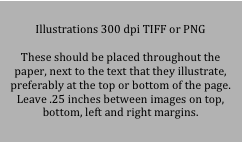
\includegraphics[width=3.31in]{figure.png}
%\caption{This is an example of figure caption. Note that all figures, and tables are to be referenced in the text. \copyright Respect Copyright.}
%\end{figure}
